% !TeX spellcheck = en_US
\addscenariosection{1}{Clash Scenario}{Dragoncurse Castle}{\images/frenzy.png}

\begin{multicols*}{2}

\textbf{Author:} profmamadu

\textbf{Source:} \href{https://discord.com/channels/740870068178649108/1253016693517717714/1253016693517717714}{Archon Studios Discord}

\textit{The majestic castle on the hill overlooks this rich province, and the local ruler is temporarily missing, leaving only his army to defend the castle walls.
Both neighboring rulers suddenly decide that these lands are theirs by right and must be secured before the local ruler returns.
However, legend speaks of a wild dragon bound to this land.
Will you dismiss the curse as a mere distraction, or can the dragon be tamed to give you the necessary edge over your opponent?
}

\subsection*{\MakeUppercase{Scenario Length}}

This Scenario is played over a maximum of 11 Rounds.

\subsection*{\MakeUppercase{Player Setup}}

\textbf{Player Count:} 2

\textbf{Starting Resources:} 20 \svg{gold}, 4 \svg{building_materials}, 2 \svg{valuables}

\textbf{Starting Income:} 15 \svg{gold}, 2 \svg{building_materials}, 1 \svg{valuables}

\textbf{Starting Units:}
\begin{itemize}
  \item 2 × A Pack \svgunit{bronze} Units with the lowest Recruitment cost
\end{itemize}

\textbf{Town Buildings:} \svgunit{bronze} Dwelling

\textbf{Map Tile Pool:} None

\textbf{Additional Bonus:} None

\subsection*{\MakeUppercase{Map Setup}}
Take the following Map Tiles and arrange them as shown in the Scenario map layout:
\begin{itemize}
  \item 2 × Starting (I) Map Tile
  \item 2 × Far (II-III) Map Tile
  \item 5 × Near (IV-V) Map Tile
  \item 2 × Center (VI-VII) Map Tiles, blindly choosing one with the Random Town Field and the other with a Dragon Utopia Field.
\end{itemize}

\subsection*{\MakeUppercase{Victory Conditions}}
When the Random Town is captured for the first time, players continue playing the current Round and then play \textbf{one additional final Round}.
The player controlling the Random Town at the end of that final Round is the winner.

\subsection*{\MakeUppercase{Defeat Conditions}}
At the end of the \nth{10} Round, if no player controls the Random Town, both players lose the game (\textit{the local ruler returns to the castle and regains control of the province}).
However, if the Random Town is first captured in the \nth{10} Round, the game proceeds as normal to its additional final Round (in this case, the \nth{11} Round).

\subsection*{\MakeUppercase{Timed Events}}

  \textbf{\nth{4} and \nth{8} Round:}
\begin{itemize}
  \item Remove all Black Cubes from Water Wheels and Windmills on the map.
  \item All Heroes gain +1 \svgeven{movement}
\end{itemize}

\end{multicols*}

\begin{multicols}{2}
\subsection*{\MakeUppercase{Additional Rules}}
During this Scenario:
\begin{itemize}
  \item Whenever an Obelisk is Visited for the first time, the Visiting player gains 2 \svg{building_materials}
  \item The Random Town is defended by Walls and a Gate when owned by a player, but it only has an Arrow Tower if that player already has a Citadel.
  \item Like any other Town, when the Random Town is owned by a player, it is a valid location for that player to:
    \begin{itemize}
      \item Place a newly Recruited Secondary Hero.
      \item Place the Main Hero when defeated.
      \item Temporarily transport the army to, for 8 \svg{gold}, when the Random Town is attacked.
    \end{itemize}
  \item The first player to Visit the Dragon Utopia (after defeating the defending Azure Unit(s)) draws Cards from the Neutral Units \svgunit{azure} Deck until a Dragon not associated with any Faction is drawn.
    The player may immediately Recruit that Dragon for free.
\end{itemize}

\columnbreak

\phantom{.}
\vfill
\begin{center}
  \transparent{0.3}{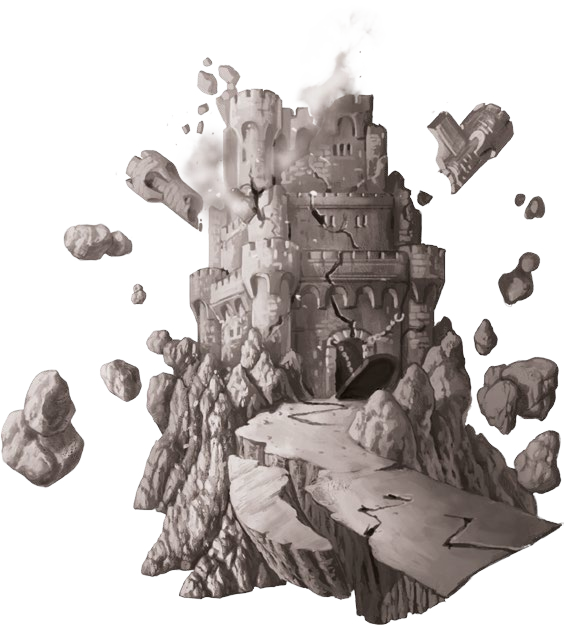
\includegraphics[width=\linewidth, keepaspectratio]{\images/earthquake.png}}
\end{center}
\vfill
\phantom{.}
\end{multicols}

\begin{tikzpicture}[overlay]
  \centering
  \node at (8.5, -4) {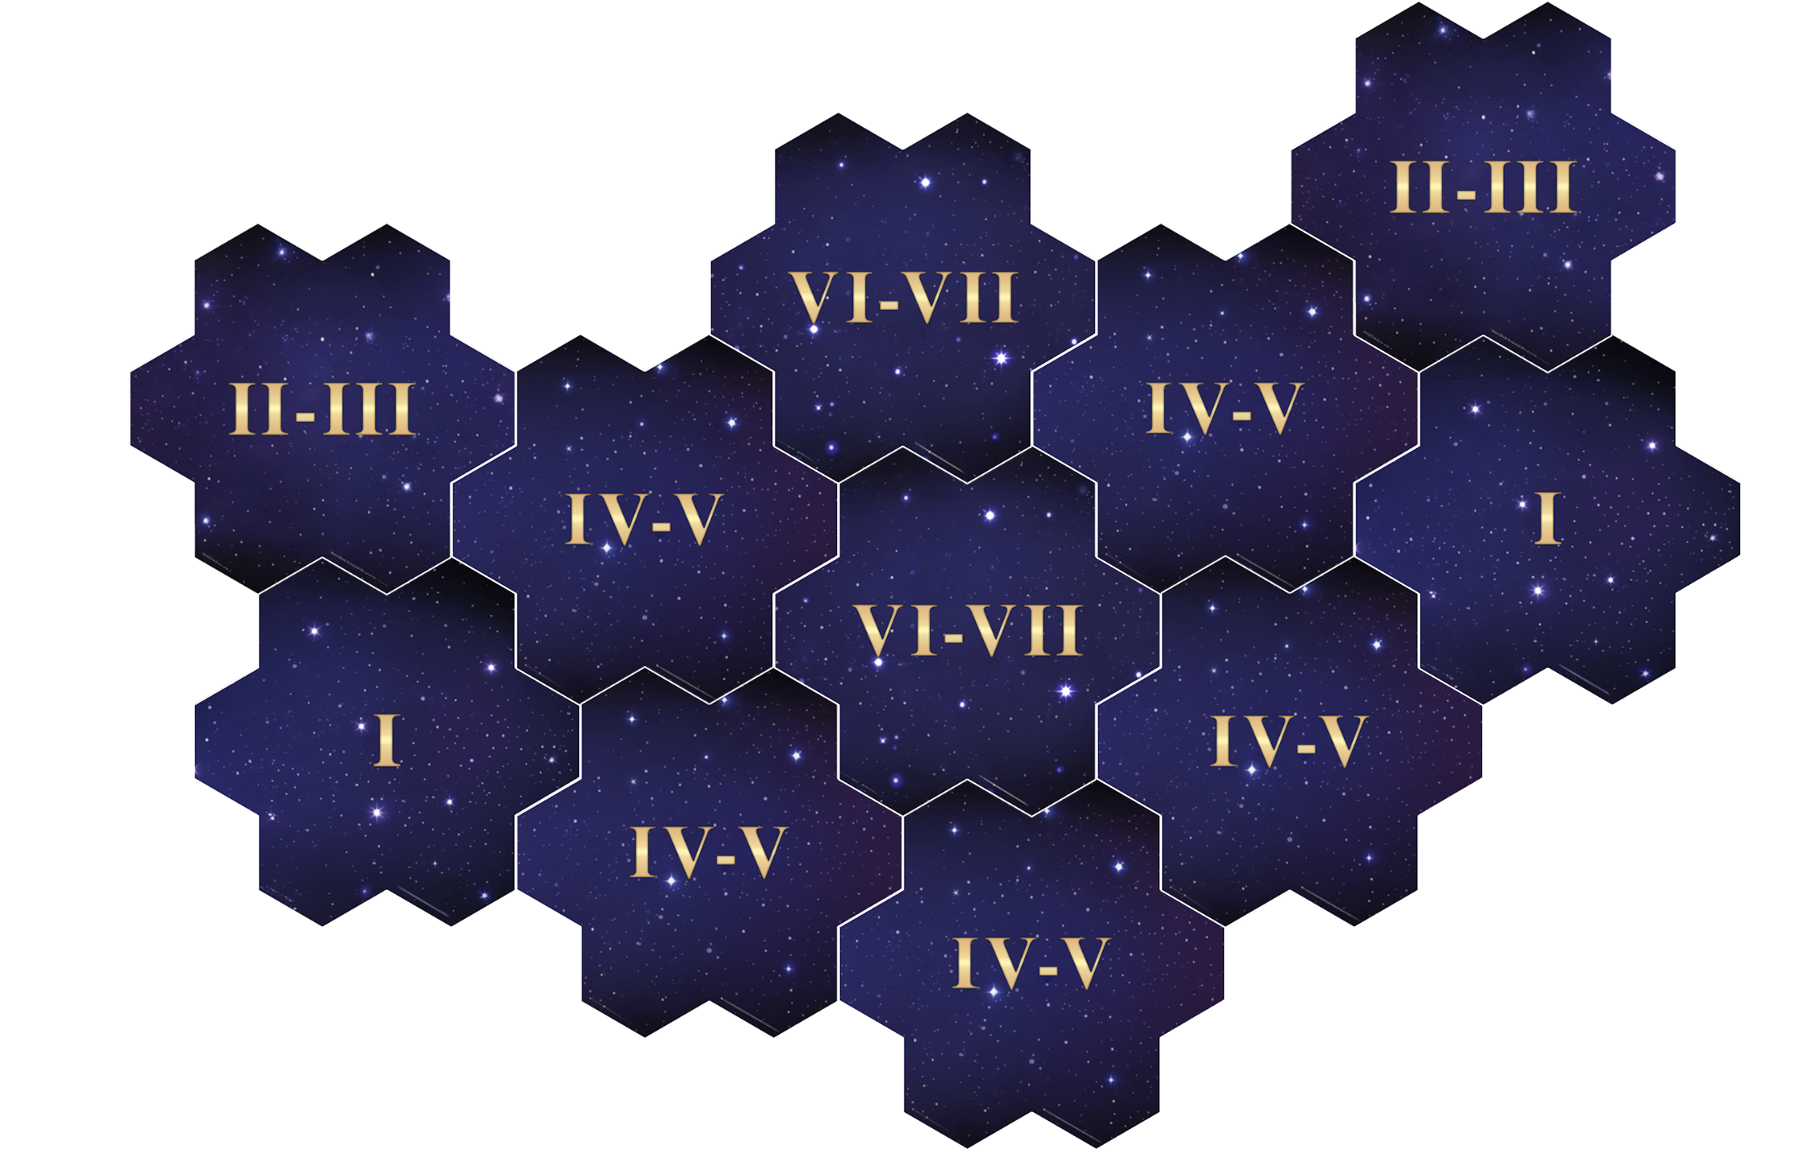
\includegraphics[width=0.7\paperwidth]{\maps/dragoncurse-castle.png}};
\end{tikzpicture}

